\setchapterpreamble[u]{\margintoc}
\chapter{Flavour Composition Analysis}
\labch{analysis}
Using the on the event sample (HESE) introduced in the previous chapter, where each event is reconstructed into one of three distinct morphologies (Single Cascades, Tracks and Double Cascades), a flavour measurement of the high energy diffuse neutrino spectrum can be performed. This chapter focuses on the methods and various components of this flavour measurement. 

The chapter begins by detailing these statistical techniques, with a focus on forward folding likelihood fits, which plays a crucial role in distinguishing signal from background and identifying flavour contributions. In addition, different components and parameters introduced (or modified) in this iteration of the analysis are explained subsequently. Following this, the software used to perform the fit is discussed in detail. Finally, the chapter evaluates the sensitivity of the analysis, providing estimates of detection limits and the potential to constrain key physical parameters within the context of neutrino flavour identification.

\section{Analysis Method}
\label{sec:analysis}
This analysis utilizes a binned maximum likelihood estimation (MLE) approach to perform statistical inferences on observed data. Binning the data offers computational efficiency by reducing the dimensionality of the problem, allowing for quicker calculations of likelihoods over a range of model parameters. Each analysis bin contains data points that represent a specific range of measured quantities, such as energy or angular distributions.

To incorporate the complexities of detector response and model uncertainties, the concept of forward folding is employed. Forward folding integrates theoretical model predictions with the response of the detector, producing expected distributions that can be directly compared to the binned observed data. This method allows for the inclusion of different flux models, systematic uncertainties, and detector efficiencies, all folded into the predicted likelihood. As a result, this approach enables robust and precise inference of underlying physical parameters, particularly in the context of high-energy astrophysics, where signal and background differentiation is challenging.

\subsection{Binned Maximum-likelihood Fits}
\label{sec:MLE}
When fitting a data sample with a large size (large $N$), it is common practice to bin the data in order to enhance the computational efficiency of the likelihood function calculation. This binning procedure groups the data into discrete intervals, or \emph{bins}, based on one or more \emph{observables}, such as energy or zenith. This simplification is not harmful as long as the variation of the probability density function (PDF), $f(x|\theta)$, within each bin is insignificant compared to its variation across all the bins. In other words, the binning should not discard crucial information about the parameter vector $\theta$ that governs the underlying physical model. If binning is applied appropriately, the process retains the ability to accurately infer the parameters of interest while significantly speeding up the computational process, particularly in high-dimensional analyses where unbinned likelihood fits may be computationally prohibitive.

The binned likelihood method works by comparing the number of observed events in each bin to the expected number of events, which are typically predicted through Monte Carlo simulations. In the analysis, these Monte Carlo templates are created for various theoretical flux components, such as astrophysical, atmospheric etc. for both signals or background. Each template provides a predicted event distribution based on specific values of the \emph{signal} parameters $\theta$ along with \emph{nuisance} parameters, $\xi$, which describe the physical processes being studied. These templates are then forward folded, meaning they incorporate the effects of the detector response, before being compared to the observed data. By adjusting the model parameters, the predicted event counts in each bin can be varied to find the \emph{best fit} to the data. The number of observed events $n$, in each bin $i$ ($n_i$), is assumed to follow a Poisson distribution \sidecite{data_analysis_book}. The expected number of events in bin $i$, $\mu_i(\theta,\xi)$, represents the sum of contributions from all signal and background components. The Poisson likelihood for a given bin is defined as:

\begin{equation}\label{eq:Poisson}
    P(n_i|\mu_i(\theta,\xi)) = \frac{\mu_i(\theta,\xi)^{n_i} e^{-\mu_i(\theta,\xi)}}{n_i!}
\end{equation}

where $\mu_i(\theta,\xi)$ is the expected number of events in bin $i$ and $n_i$ is the observed number. The total likelihood for the entire dataset is then the product of the likelihoods for all bins:

\begin{equation}\label{eq:llh_noprior}
    \mathcal{L}(n|\mu_i(\theta,\xi)) = \prod_{i=1}^{N} P(n_i|\mu_i(\theta,\xi))
\end{equation}

Incorporating systematic uncertainties into the likelihood function is crucial for obtaining realistic results, as these uncertainties often arise from imperfect detector calibration or background estimations. Such systematic uncertainties are modeled as nuisance parameters in the likelihood fit. These parameters are typically constrained by prior knowledge and treated as additional variables in the fitting process. For each of the $k$ nuisance parameters, $\xi_j$, a Gaussian prior is introduced, penalizing deviations from the central value $\bar{\xi_j}$ by an amount proportional to the known uncertainty $\sigma_{\xi_j}$, changing the likeli:

\begin{equation}\label{eq:llh_withprior}
    \mathcal{L}(n|\mu_i(\theta,\xi)) = \prod_{i=1}^{N} P(n_i|\mu_i(\theta,\xi)) \prod_{j=1}^{k} \exp\left(-\frac{1}{2}\left(\frac{\xi_j - \bar{\xi_j}}{\sigma_{\xi_j}}\right)^2\right)
\end{equation}
By maximizing this likelihood, the best-fit parameters $\theta$ can be found. In practice, the fit is performed by minimizing $-\ln\mathcal{L}$, as it simplifies the computation (see \ref{eq:logllh}). 

\begin{equation}\label{eq:logllh}
    \ln(\mathcal{L}(n|\mu_i(\theta,\xi))) = \sum_{i=1}^{N} \left[ n_i \ln(\mu_i) - \ln(n_i!) - \mu_i \right] 
    - \sum_{j=1}^{k} \frac{1}{2} \left( \frac{\xi_j - \bar{\xi_j}}{\sigma_{\xi_j}} \right)^2
\end{equation}

This modified likelihood is often referred to as the \textbf{profile likelihood}, as it profiles over the nuisance parameters by marginalizing or constraining them using prior information.

Once the likelihood function is constructed, the next step is hypothesis testing. A specific model hypothesis can be tested by using a likelihood ratio test. The likelihood ratio compares two hypotheses: the test model (with parameters $\theta_t$) and the best-fit model (with parameters $\hat{\theta}$):

\begin{equation}\label{eq:llh_ratio_TS}
    -2 \Delta \ln \mathcal{L} = -2 \ln \left( \frac{\mathcal{L}(n|\mu(\theta_t, \xi_t))}{\mathcal{L}(n|\mu(\hat{\theta}, \hat{\xi}))} \right)
\end{equation}

The factor $-2$ is included for convenience, as it allows the test statistic to follow a $\chi^2$-distribution, according to Wilks' theorem \sidecite{Wilks_thm}. This enables the calculation of confidence levels (CL) of the parameter of interest without the need for computationally expensive Monte Carlo simulations. However, Wilks’ theorem is only valid when the dataset is large and the model parameters are unbounded. If either condition is not met, the test statistic may deviate from a $\chi^2$-distribution, necessitating the use of Monte Carlo pseudo-experiments to determine the confidence intervals via the so-called \emph{Feldman Cousins} method \sidecite{feldman_cousin}, with an extension to incorporate nuisance parameters \sidecite{feldman_cousin_nuisance,asimov}.

The test statistic derived from the likelihood ratio can be used to construct confidence regions for the parameters of interest. For instance, in one-dimensional parameter scans, the confidence interval is obtained by comparing the test statistic to the cumulative distribution of a $\chi^2$-distribution with one degree of freedom. When scanning over two or more parameters, a multi-dimensional profile likelihood scan is required, which significantly increases the computational complexity. In some cases, the Asimov dataset \cite{asimov}—a single dataset representing the median outcome of many pseudo experiments—can be used to estimate the median sensitivity of the analysis. This method provides an efficient way to estimate confidence intervals and test the sensitivity of the analysis without the need for exhaustive Monte Carlo trials. Asimov dataset and Wilks' theorem are both used to derive sensitivity presented in \ref{sec:sensitivty}. It is important to point out that the primary parameter of interest in this analysis is the astrophysical neutrino flavour fractions, which are constrained to be non-negative ($\phi_{\nu_\tau} \geq 0$) and limited by the small number of observed double cascade events. As a result, the applicability of Wilks' theorem is evaluated as needed.

\subsection{SAY Likelihood}
\label{sec:SAY}

The likelihood construction described in section \ref{sec:MLE} relies on the Poisson likelihood, which assumes that the expectations for each bin, $\mu_i$, are known exactly. This assumption holds when the Monte Carlo simulations used in generating the expected distributions have large statistics. However, MC simulations inherently come with their own uncertainties due to finite statistics, particularly in bins with lower event counts.

In binned forward-folding fits, statistical inferences are made by comparing observed data counts in each bin to the expected counts derived from the simulations. As outlined in Equation~\ref{eq:Poisson}, the Poisson likelihood assumes that $\mu_i$, the expected value per bin, is well-determined. However, this is often not the case in analyses like ours, where overall event rates are low, and individual bin expectations may fluctuate significantly due to limited MC statistics. This mismatch can lead to deviations between the observed data and MC predictions if these fluctuations in $\mu_i$ are not correctly accounted for.

To address this issue, an extended form of the Poisson likelihood ($\mathcal{L}_{\mathrm{eff}}$), or the so-called \textbf{SAY likelihood}, is used in this analysis \sidecite{SAY}. This likelihood incorporates the uncertainty from the limited MC statistics and provides more appropriate coverage of the expected $\mu_i$ values. Specifically, the distribution of MC event weights in each bin is corrected using a scaled Poisson distribution, which introduces an additional uncertainty term, $\sigma_j^2$, for each bin. This term depends on the weights $w_i^j$ of the MC events in the $j$-th bin and is defined as:

\begin{equation}
\sigma_j^2 = \sum_{i} (w_i^j)^2
\end{equation}

This uncertainty term, $\sigma_j^2$, is larger in bins with low statistics, and smaller in bins with higher statistics, ensuring that fluctuations in low-stat bins are adequately covered. This formalism results in more conservative limits, with generally wider contours for the final result, as the additional statistical uncertainty is incorporated into the fit. One limitation of this approach is that the Asimov dataset \sidecite{asimov}, described in the previous section, is not applicable with the SAY likelihood. This is because the $\sigma_j$ term can significantly alter $\mu_i$ in each bin, making it impossible to recover the injected model parameters. As a result, deviations from injected values may appear, especially in cases like the \texttt{MuonGun}, discussed in the next section. Alternatively, the standard Poisson likelihood can be used, though the resulting limits may be less conservative than the reality accounted for by the SAY likelihood.


\section{Components of the fit}
\label{sec:components}
The choice of the likelihood function and its subsequent requirement  was outlined in the previous section. In this section, the focus shall be on the actual construction of the likelihood and the essential components involved. The construction proceeds as follows:

\begin{enumerate}
    \item The parameters to be measured, known as \emph{signal parameters} (denoted by $\theta$), along with all \emph{nuisance parameters} ($\xi$), which may originate from detector systematics or background modeling (such as atmospheric spectra), are identified and bounded where necessary.
   
    \item These parameters are applied in the form of the neutrino \emph{flux}, assigning each Monte Carlo event a specific \emph{weight} based on the individual fluxes.

    \item A set of observables that are most sensitive to the signal parameters, such as astrophysical neutrino fluxes, is selected and appropriately binned for analysis.
    \marginnote{
        \begin{kaobox} 
        This is why a penalty term is introduced in the likelihood. A Gaussian prior ensures that the parameters remain within the $1\sigma$ prior region, penalizing the likelihood if the fit favors values outside this range. 
        \end{kaobox}}
    \item The experiment is performed, and the observed data events $n$ are sorted into the predefined bins of the analysis histograms. A fit is conducted by varying each of the parameters (and, consequently, the fluxes) until the observed data events are optimally described. 
\end{enumerate}


\subsection{Model parameters}
\label{sec:params}
All the model parameters used in the fit, along with which fluxes they affect, are listed in \reftab{fit_params}. The model parameters consist of either flux components (astrophysical or atmospheric) or detector systematics. Baseline models and their corresponding values, wherever applicable, are specified for each parameter, along with the choice of priors. The astrophysical flux parameters represent the high-energy neutrino contributions from distant sources, while atmospheric flux models account for neutrinos originating from cosmic ray interactions within in atmosphere of Earth. Detector systematics reflect uncertainties in detector performance. 

\begin{table*}[h]
    \caption{Parameters used in the likelihood desribed in Equation \ref{eq:llh_withprior}. The gaussian priors on the parameters (if applicable) in terms of the mean ($\mu$) and width ($\sigma$) are stated on the alongside.}
    \labtab{fit_params}
    
    \begin{tabular}{ |c |c|}
        \hline
        Parameter & Prior ($\mu,\sigma$)\\
        \hline
        \hline
        \multicolumn{2}{c}{\textbf{Astrophysical Flux (Signal) Parameters}}\\
        \hline
        astro. $\nu_{\mu}$ normalisation [$10^{-18} \mathrm{GeV}^{-1}\mathrm{cm}^{-2}\mathrm{sr}^{-1}\mathrm{s}^{-1}$]($\phi_{\nu_{\mu}}$) & - \\
        % \hline
        astro. spectral index ($\gamma_{\mathrm{astro}}$) & -\\
        % \hline
        scaling factor to modify total flux norm ($\Phi_{\nu+\bar\nu}^{\mathrm{astro}}$) relative to $\phi_{\nu_{\mu}}$ ($s_{\nu_e}$ astro. $\nu_{e}$)&- \\
        % \hline
        astro. $\nu_{\tau}$ scaling factor to modify total flux norm ($\Phi_{\nu+\bar\nu}^{\mathrm{astro}}$) relative to $\phi_{\nu_{\mu}}$ ($s_{\nu_{\tau}}$) & -\\
        \hline
        \multicolumn{2}{c}{\textbf{Atmospheric Flux Systematics}}\\
        \hline
        Conventional Flux normalisation ($\Phi_{\mathrm{conv}}$)  & (1.0,0.2)\\
        % \hline
        Prompt Flux Normalisation ($\Phi_{\mathrm{prompt}}$) &  - \\
        % \hline
        Interpolation between Cosmic Ray Models ($\xi_{\mathrm{CR}}$)  & (0,1)\\
        % \hline
        Cosmic Ray Spectral Index Shift ($\Delta\gamma_{\mathrm{CR}}$) &  (0,0.05)\\
        % \hline
        Barr-parameter modifying the pion-contribution ($H_{\mathrm{Barr}}$) & (0,0.15)\\
        % \hline
        Barr-parameter modifying the kaon-contribution ($W_{\mathrm{Barr}}$) & (0,0.40)\\
        % \hline
        Barr-parameter modifying the pion-contribution ($Y_{\mathrm{Barr}}$)& (0,0.30)\\
        % \hline
        Barr-parameter modifying the pion-contribution ($Z_{\mathrm{Barr}}$) & (0,0.12)\\
        % \hline
        Muon Flux Normalisation ($\Phi_{\mathrm{muongun}}$)  & (1,0.5)\\
        % \hline
        Scale factor for Neutrino Nucleon Inelasticity weight ($\mathrm{I}_{\mathrm{scale}}$) & (1,0.1)\\
        \hline
        
        \multicolumn{2}{c}{\textbf{Detector Systematics}}\\
        \hline
        Optical Efficiency of DOMs ($\eta_{\mathrm{domeff}}$) & (1.0,0.1)\\
        % \hline
        Ice Absorption Scaling ($\eta_{\mathrm{abs}}$)  & (1.0,0.05)\\
        % \hline
        Ice Scattering Scaling ($\eta_{\mathrm{scat}}$) & (1.0,0.05)\\
        % \hline
        Parametrization for refrozen icecolumn ($\eta_{\mathrm{h.ice-p0}}$)  & (-0.27,0.5)\\
        % \hline
        Parametrization for refrozen icecolumn ($\eta_{\mathrm{h.ice-p1}}$) & (-0.042,0.05)\\
        % \hline
        Ice Anisotropy Scaling ($\eta_{\mathrm{aniso}}$) &  -\\
        \hline
        \hline
    \end{tabular}
    
\end{table*}

\newpage
\textbf{The flux of astrophysical neutrinos} is modeled as a single power law of the form
\begin{equation}\label{eq:SPL}
\Phi_{\nu + \bar{\nu}}^{\mathrm{astro}} = \Phi_{\mathrm{0}}^{\mathrm{astro}} \times 
    (1 + s_{\nu_{e}} + s_{\nu_{\tau}}) \times
    \left( \frac{E_\nu}{\mathrm{100\,TeV}} \right)^{-\gamma_{\mathrm{astro}}}
\end{equation}
where $\gamma_{\mathrm{astro}}$ is the spectral index, $E_\nu$ is the neutrino energy, and $\Phi_{\nu + \bar{\nu}}^{\mathrm{astro}}$ is the all-flavor (including particle and anti-particle) normalization. Two scaling factors, $s_{\nu_{e}}$ and $s_{\nu_{\tau}}$, modify the flux of electron and tau neutrinos relative to the muon neutrino flux $\Phi_{\mathrm{0}}$. These scaling factors help determine the flavour ratio $\nu_e:\nu_{\mu}:\nu_{\tau}$ as:

\begin{equation}\label{eq:flav_frac}
    \begin{array}{rcl}
        f_{e} = \frac{s_{\nu_{e}}}{(1 + s_{\nu_{e}} + s_{\nu_{\tau}})}, \quad
        f_{\mu} = \frac{1}{(1 + s_{\nu_{e}} + s_{\nu_{\tau}})}, \quad
        f_{\tau} = \frac{s_{\nu_{\tau}}}{(1 + s_{\nu_{e}} + s_{\nu_{\tau}})}
    \end{array}
\end{equation}

The signal parameters for the flavor analysis are these two scaling factors, $\Phi_{\mathrm{0}}$, and $\gamma_{\mathrm{astro}}$. All other subsequent parameters explained are the nuisance parameters. In Eq.~\ref{eq:SPL}, it is assumed that each flavor has an identical spectral shape ($\gamma_{\mathrm{astro}}$). This assumption is justified because the HESE sample used in this analysis is small and has limited power to constrain individual spectra for each flavor. For the sensitivity study described in \ref{sec:sensitivity}, the benchmark spectral parameter values are taken from the previous iteration of this analysis \sidecite{HESE7_sample}, with $\gamma_{\mathrm{astro}} = 2.87$ and $\Phi_{\mathrm{0}} = 2.12 \times 10^{-18} \mathrm{GeV}^{-1}\ \mathrm{cm}^{-2}\ \mathrm{sr}^{-1}\ \mathrm{s}^{-1}$ assuming an equipartition of flavor ratios (i.e., $\nu_e : \nu_{\mu} : \nu_{\tau} = 1:1:1$).

\textbf{Atmospheric flux components} are constrained by priors because they are more accurately measured with other IceCube data samples. The high-energy starting event selection is very efficient in reducing atmospheric muons due to the veto requirement and the down-going atmospheric neutrinos from the same cosmic-ray-induced air shower, thanks to the self-veto effect.

Depending on the parent hadron type, the atmospheric neutrino flux is divided into two components: \textbf{Conventional neutrino flux} (produced via decay of charged pions and kaons) and \textbf{Prompt Neutrino Flux} (produced via decay of charmed mesons). The various models of atmospheric neutrino fluxes are detailed in \ref{sec:atm_nu}. The atmospheric neutrino contribution is modeled using the Matrix Cascade Equation Solver (MCEq) \sidecite{MCEq}. The baseline primary cosmic-ray model for this calculation is H4a \sidecite{gaisser_H4a}, combined with a hadronic interaction model \texttt{SIBYLL2.3c} \sidecite{SIBYLL23c}, introducing conventional ($\Phi_{\mathrm{conv}}$) and prompt ($\Phi_{\mathrm{prompt}}$) flux normalizations to account for background contributions from these fluxes. Additionally, they are folded with the generalized self-veto probability, as described in \ref{sec:HESE}, to account for the reduced rate of atmospheric neutrinos accompanying vetoed muons from the same cosmic-ray-induced air shower. Other nuisance parameters modifying the shape of these spectra include $\xi_{\mathrm{CR}}$, which interpolates between two primary cosmic-ray models H4a and GST (see section \ref{sec:atm_nu}), an approach similar to \sidecite{diffusenumu}. The cosmic-ray model uncertainty is critical in this analysis, as it is the largest source of uncertainty in the overall atmospheric background. Furthermore, $\Delta\gamma_{\mathrm{CR}}$ accounts for corrections in the spectral index of the primary cosmic-ray spectrum, following \sidecite{hans_thesis}. Uncertainties in the hadronic interaction models, due to various $\pi$ and $K$ production cross-sections in different energy phases, introduce energy-dependent variations in atmospheric flux expectations \sidecite{Barr}. These nuisance parameters, referred to as \emph{Barr} parameters, are computed as described in \sidecite{Anatoli_HI_model}. A detailed discussion on implementing these parameters within the software framework can be found in \sidecite{richard_thesis}.

As mentioned, the veto and charge/energy cuts effectively reduce atmospheric neutrinos. However, high-energy single muons can still enter the detector, contaminating the sample. A separate nuisance parameter, $\Phi_{\mathrm{muongun}}$, is included in the fit to account for these muons. \textbf{The atmospheric Muon Flux} component is constrained by a prior partially derived from experimental data. The spectral shape is determined using a dedicated simulation that produces a flux of single muons reaching the detector (\texttt{MUONGUN}, described in \ref{sec:mc_sim}), weighted assuming the same baseline models used for atmospheric spectra (H4a). A pure-proton composition is chosen for these muons as it contributes the highest energy single muons. The normalization is estimated using the tagging method described in \cite{HESE7_sample}. A prior derived from this study is applied in this analysis. The sensitive energy range of this analysis is high, and the sample is specifically designed to minimize background contamination from atmospheric neutrinos and muons (see Section \ref{sec:HESE}). The available \texttt{MUONGUN} Monte Carlo was generated for various other IceCube analyses, that targeted lower energies as well, where background contributions are significantly higher. Most Monte Carlo events do not pass the strict cuts of this analysis, with no events at all in the cascade and double cascade bins (see \reffig{cascade_mc} and \reffig{double_mc}). Consequently, the statistical uncertainty on this component is high, requiring a Kernel Density Estimate (KDE) template for smoothing.

The remaining nuisance parameters are those arising from the imperfect knowledge of the detector components, such as the Digital Optical Modules (DOMs, see section \ref{sec:DOM}), and the detection medium, which includes both the bulk ice and hole ice models (see section \ref{sec:icemodel}), known from here-on as \textbf{Detector Systematics}. These detector systematics introduce uncertainties that can affect both the threshold and the shape of observable distributions, thereby altering the expected event rates from different flux components. Unlike previous iterations of this analysis \sidecite{marcel_thesis,Juliana_thesis}, which relied on discrete Monte Carlo sets with different values for systematics that significantly impacted the analysis observables, the current approach uses the SnowStorm simulation technique (see section \ref{sec:}). The SnowStorm method \sidecite{snowstorm} captures the full range of detector systematic variations in a single Monte Carlo dataset, avoiding the need for generating multiple datasets. It uses a first-order Taylor expansion of the observables, such as event counts in each bin, with respect to the detector systematics. The resulting gradient, called \emph{the nuisance gradient} ($\vec{G}$), allows for efficient computation of observable values as these systematic parameters vary. The expectation value of per bin event count $\mu$, for nuisance parameter variations $\vec{\eta}$ is given as,

\begin{equation}\label{eq:gradient}
    \mu(\vec{\eta})  = \mu_{\mathrm{baseline}} + \vec{\eta}.\vec{G}
\end{equation}

where, $\mu_{\mathrm{baseline}}$ is the expectation value of per bin count at basleine values of all detector systematic parameters (baseline values are the central value at which simulation was generated), when $\vec{\eta}=\vec{0}$. For this approach to be valid, it assumes that systematic effects are small enough to be treated perturbatively, allowing for a linear approximation. By marginalizing over the full ensemble of systematic variations, the prediction converges to that of the central model, effectively neglecting second-order effects. Because the dataset itself have finite statistics, appropriate uncertainty propagation is applied to the nuisance gradient (see \sidecite{richard_thesis} for details of calculations of this gradient, their uncertainties and incorporation within such fits). 

For each analysis bin, both the expected number of events and the associated variance are computed. However, two important caveats should be noted with this method. First, the gradients are calculated based on a specific flux assumption\sidenote{For the analysis presented in this thesis, the gradients are computed using the best-fit values from the HESE-7.5 year analysis \cite{HESE7_sample}, with $\gamma_{\mathrm{astro}}=2.87$, the per-flavour flux normalization $\Phi_{\nu + \bar{\nu}}^{\mathrm{astro}}=2.12$, and an equipartition among all three flavour fluxes.} and are not recalculated at every minimization step. This significantly reduces the computational time of the minimization process but may introduce inaccuracies if the assumed fluxes deviate significantly from the true values in nature, which could substantially alter the resulting gradients. A potential solution is to compute the gradients over a range of flux assumptions to check for significant deviations in the results. The second caveat arises because the expected event counts per bin, calculated using the gradients as shown in Equation \ref{eq:gradient}, are applied as an \emph{additive} correction to the overall flux expectation. Since the gradient is a vector, it can also take negative values. For softer spectra and the limited statistics of the HESE sample, this can result in negative bin counts when the expected values approach zero. This presents a problem for the likelihood fit used in the analysis, as the logarithm of a negative number cannot be computed (which the fitter will attempt to do at some point; see Equation \ref{eq:logllh}). To avoid this numerical issue, the expectation value calculated via the gradients is clipped at $\mu = 0 + \epsilon$. This ad hoc correction is justified because, although $\mu_{\mathrm{baseline}}$ may be zero in these bins, there remains significant statistical uncertainty, which typically dominates over the systematic variations.

The aforementioned gradient, can be constructed using all or part of detector systematics simulated within the snowstrom ensemble. For the analysis presented in this thesis, it is constructed using 6 parameters, listed in the \reftab{fit_params}. 
\begin{description}
    \item [\textbf{The DOM Efficiency ($\eta_{\mathrm{domeff}}$)}] accounts for factors like the quantum efficiency of the PMT and shadowing by attached cables, reducing the efficiency by 1\%. The overall uncertainty is estimated at $\pm10\%$. This impacts the reconstructed energy, as lower efficiency underestimates the photon light yield. This effect is relevant in the analysis, as it shifts the energy distribution across bins and the energy thresholds in particular.
    \item [\textbf{Absorption ($\eta_{\mathrm{abs}}$) and Scattering ($\eta_{\mathrm{scat}}$) Scaling}] accounts for variations in scattering and absorprion coefficients of ice mapped across depth grid of the south pole ice. The baseline model for this mapping is SPICE-3.2.1, with priors set to a 5\% width around the central value, based on the uncertainty derived from calibration data obtained using flasher LEDs.. An increase in scattering coefficients extends the photon scattering path, increasing the chance of absorption before detection. Variations in ice scattering and absorption mainly affect energy reconstruction and may introduce minor directional bias, with the energy shift being the primary concern in this analysis.  
    \item [\textbf{hole ice parameters ($\eta_{\mathrm{h.ice-p0}}$ and $\eta_{\mathrm{h.ice-p1}}$)}] accounts for the differences in optical properties between the refrozen ice in the DOM deployment columns and the surrounding bulk ice. Uncertainties and priors are based on a recent study that analyzed flasher data \sidecite{holeice_eller_icrc23}.
    \item [\textbf{Ice anistropy}] discussed in detail in sections \ref{sec:icemodel} and \ref{sec:icemodel_checks} affects the double cascade reconstruction greatly. For the icemodel used in simulation, this parameter is modelled as a modulation of the nominal scattering coefficient, analogous to thay used in \sidecite{Juliana_paper}.
\end{description}



Lastly, an additional nuisance parameter, affecting all the neutrino fluxes (Astrophysical and atmospheric) is used that modifies overall normalisation of these fluxes, \textbf{Neutrino-Nucleon Inelasticity Scaling ($\mathrm{I}_{\mathrm{scale}}$)}. This parameter is introduced to account for  inelasticity which is a measure of the fraction of the neutrino's energy that is transferred to the hadronic system in an inelastic neutrino nucleon scattering process, mathematically given as,
\begin{equation}
     y  = \frac{E_{\text{hadron}}}{E_\nu}
\end{equation}
Mean inelasticity $\langle y \rangle$ is the average value of the inelasticity $y$ over many scattering events. It provides a statistical measure of the average fraction of the neutrino's energy that is transferred to the hadronic system. This becomes particularly relevant for the starting tracks as, $\langle y \rangle$ is energy dependednt and hence amount of energy transferred to the muon after $\nu_{\mu}$ CC interaction, will therefore be different for different energies of Neutrino (and hence different events). For this analysis, a scaling factor is introduced, which is based on formulation provided in \sidecite{gary_paper}, that allows to vary Normalisation $N$ of the inelasticity distribution, 
\begin{equation}
    \frac{dp}{dy} = N \left( 1 + \epsilon (1 - y)^2 \right) y^{\lambda - 1}
\end{equation}
where N is the normalisation given as,
\begin{equation}\label{eq:inel}
    N = \frac{\lambda (\lambda + 1) (\lambda + 2)}{2\epsilon + (\lambda + 1) (\lambda + 2)}
\end{equation}

The theoretical prediction of \(\langle y \rangle\) from the CSMS tables \sidecite{CSMS} is calculated for the mean inelasticity distribution for a given event. By fixing \(\langle y \rangle\), $\lambda$ \ref{eq:inel} is the fitted to apply a reweighting factor to \textit{scale} the inelasticity ($\mathrm{I}_{\mathrm{scale}}$). Variations are permitted within 10\% of their default value. The parameter is applied to all neutrino fluxes as it can affect any fluxes where a neutrino interacts via Deep Inelastic Scattering.

\subsection{Analysis Observables and their Distributions}
\label{sec:hists}

In forward folding fits, selecting appropriate observables is crucial for distinguishing between the signal and background hypotheses. The analysis uses all the HESE events above 60 TeV, further divided in 3 sub-samples of \emph{Single Cascades, Tracks and Double Cascades}. These 3 sub-samples are binned in 2-dimensional monte carlo templates of appropriate observables, such that bakground and signal templates are clearly distingishabe. For example, when measuring the spectrum of astrophysical neutrinos, the background consists of neutrinos from other sources, primarily atmospheric fluxes. Key observables that allow for effective differentiation between astrophysical and atmospheric neutrinos include the total deposited energy ($\mathrm{E}_\mathrm{tot}$) and the zenith angle ($\theta_{\mathrm{zenith}}$) of the interacting neutrino. The motivation for focusing on these variables stems from their distinct behavior in atmospheric and astrophysical neutrino spectra (see Section~\ref{sec:atm_nu}). In particular, down-going atmospheric neutrinos are efficiently suppressed due to the self-veto effect, while up-going atmospheric neutrinos, which cannot be reduced by this veto, become an irreducible background. 

\marginnote{
        \begin{kaobox} 
        The astrophysical spectrum that is assumed for all the monte carlo templates and sensitivity is using a single-power law based on best-fit values of HESE-7.5 years spectrum measurements \cite{HESE7_sample}, given as,
            \begin{equation}\label{eq:SPL}
                \frac{d\Phi_{\nu + \bar{\nu}}^{\mathrm{astro}}}{dE} = 6.98.10^{-18}\left( \frac{E_{\nu}}{100 \, \text{TeV}} \right)^{-2.87} 
            \end{equation}
        In units of $\text{GeV}^{-1} \, \text{cm}^{-2} \, \text{s}^{-1} \, \text{sr}^{-1}$, with flavour composition of $\nu_e:\nu_{\mu}:\nu_{\tau}=1:1:1$
        \newline
        The prompt component is missing from all templates as best-fit value of $\Phi_{\mathrm{prompt}}$ of prompt flux normalization was 0. 
        \end{kaobox}
}
For the analysis presented in this thesis, the primary goal is to measure the flavor composition of astrophysical neutrinos. A key component of this analysis, as highlighted in Section~\ref{sec:PID}, is the identification and classification of $\nu_\tau$-induced double cascade events. Note that the PID assigned is not used as a proxy to tag flavour on an individual event bases, but through statistical analyses of the overall data set, by using Monte Carlo templates. Double cascades are a signature of $\nu_\tau$ interactions, and their identification relies heavily on the observables $\mathrm{E}_\mathrm{tot}$ and the reconstructed double cascade length ($\mathrm{L}_{\text{dc}}$), which provide the most discriminatory power for separating the flavors of astrophysical neutrinos, see \reffig{LvsE_signalbkg}. All double cascade events are binned into a two-dimensional Monte Carlo template, with one axis representing the reconstructed tau decay length ($L_{\text{dc}}$) and the other representing the reconstructed total deposited energy ($E_{\text{Tot}}$). The $L_{\text{dc}}$ is divided into 10 bins ranging from 10 m to 1000 m, while $E_{\text{Tot}}$ is divided into 13 bins spanning 60 TeV to 12.6 PeV, both using logarithmic spacing, as shown in ~\reffig{LvsE_signalbkg}. It is important to note that adding a third dimension, such as energy asymmetry, offers significant discriminatory power by reducing the low-length single cascade background, enhancing the sensitivity to measure the flavor ratio \sidecite{Neha_ICRC_IC}. However, a detailed study revealed that the limited Monte Carlo statistics and small sample size of the HESE data resulted in many empty bins, which posed challenges for forward-folding fits. As a result, the third dimension was ultimately excluded from the analysis.


\begin{figure*}[h!]
    \begin{subfigure}[h]{0.72\textwidth}
        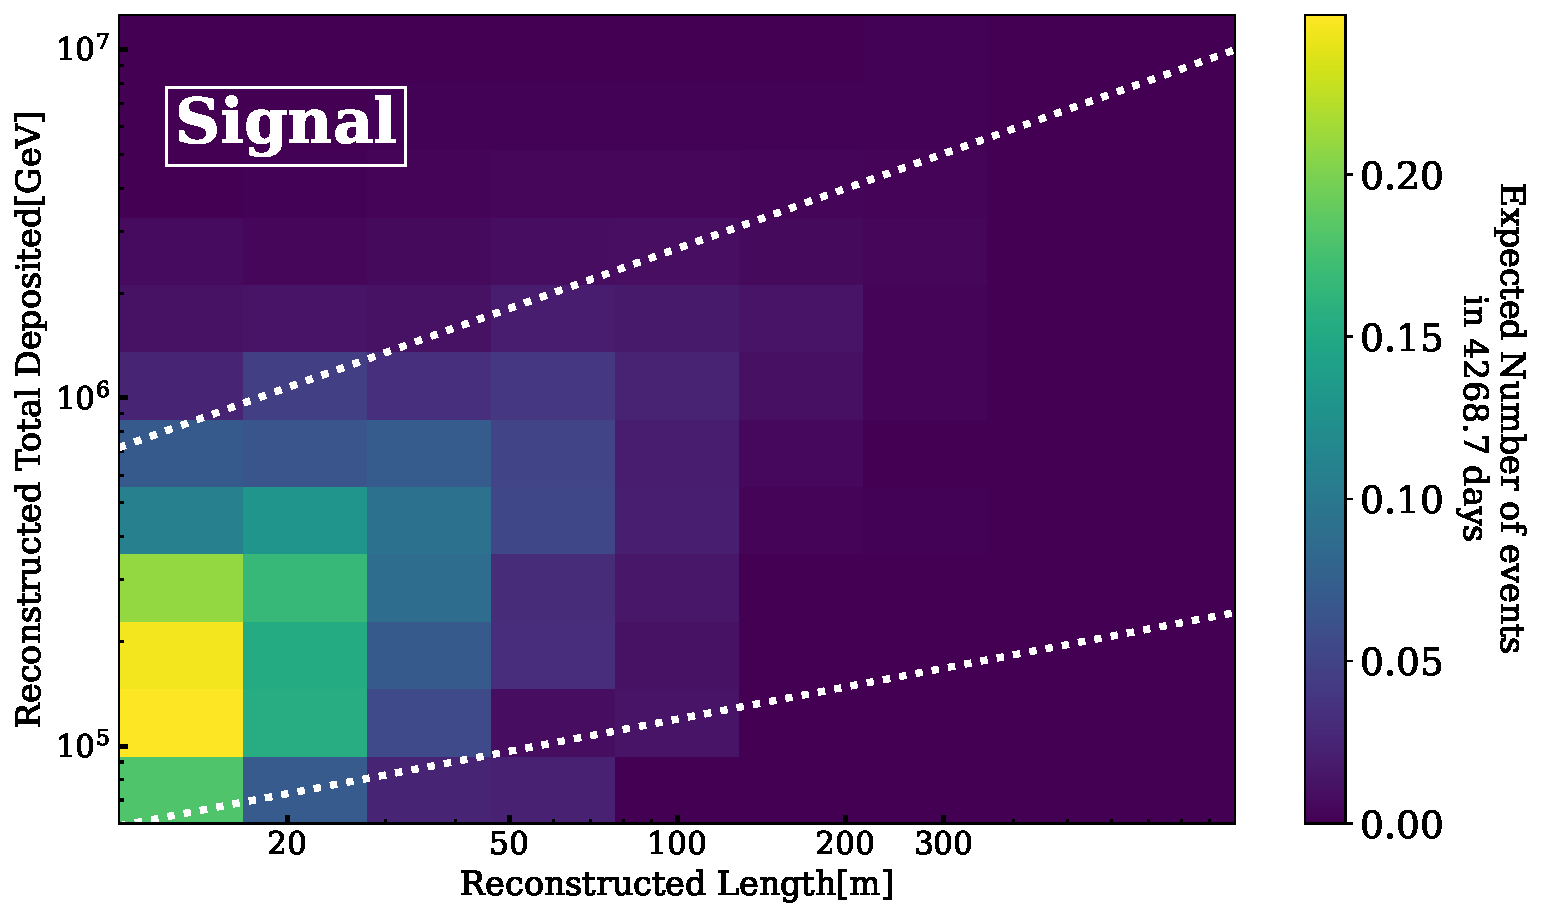
\includegraphics{./figures/Analysis/LvsE_signal.pdf}
    \end{subfigure}
    \hfill
    \begin{subfigure}[h]{0.72\textwidth}
        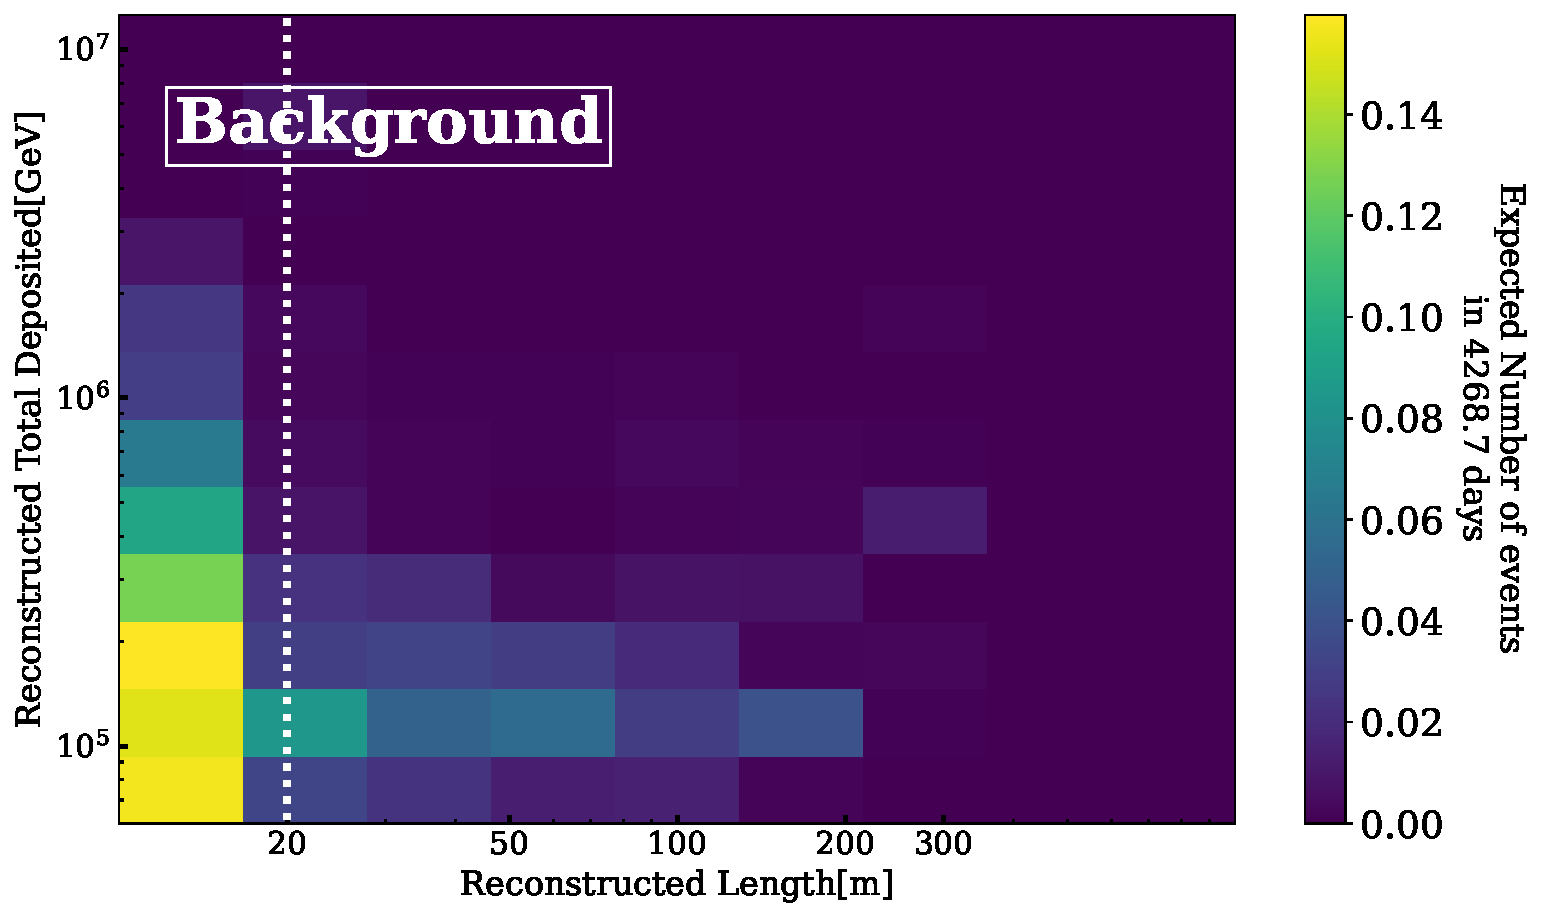
\includegraphics{./figures/Analysis/LvsE_Bkg.pdf}
       
    \end{subfigure}%
    \caption{2D Monte Carlo templates, constructed using reconstructed total energy ($E_{\text{Tot}}$) and double cascade length ($L_{\text{dc}}$) for events classified as \textbf{double cascades}. The signal (left), representing $\nu_\tau$-induced double cascades, shows a clear correlation between $L_{\text{dc}}$ and $E_{\text{tot}}$, with 68\% of events within the indicated signal region (dotted white line). In contrast, the background (right), consisting of $\nu_\mu$ and $\nu_e$ events, lacks this correlation and clusters at low $L_{\text{dc}}$, 68\% of all the background events lying below the indicated white dotted verticle line.}
    \labfig{LvsE_signalbkg}
\end{figure*}

Under the double cascade hypothesis, true single cascades are typically reconstructed with a small $\mathrm{L}_{\mathrm{dc}}$ but with most of their energy concentrated in the first cascade (with the energy asymmetry $E_A \rightarrow 1$). Hence, misclassified single cascades tend to cluster around low $\mathrm{L}_{\mathrm{dc}}$ and low $\mathrm{E}_{\mathrm{Tot}}$, with the distribution of $\mathrm{L}_{\mathrm{dc}}$ falling off rapidly, as indicated by the verticle line, on right panel of \reffig{LvsE_signalbkg}. In cases where a track is reconstructed under the double cascade hypothesis, the largest energy depositions are interpreted as the cascade vertices, leading to an arbitrary $\mathrm{L}_{\mathrm{dc}}$ value. These tracks, when misclassified as double cascades, typically exhibit low $\mathrm{E}_{\mathrm{Tot}}$, consistent with the falling astrophysical spectrum. This is too visible in right panel of \reffig{LvsE_signalbkg}.

True double cascades from $\nu_\tau$-CC interactions, on the other hand, exhibit a strong correlation between $\mathrm{L}_{\mathrm{dc}}$ and $\mathrm{E}_{\mathrm{Tot}}$, see. This correlation between $\mathrm{L}_{\mathrm{dc}}$ and $\mathrm{E}_{\mathrm{Tot}}$ is primarily used to determine the compatibility of an event with a $\nu_\tau$ interaction as opposed to another flavor. The Monte Carlo distributions (PDFs) of $\nu_\tau$-induced double cascades clearly show this correlation (see left panel of \reffig{LvsE_signalbkg}, indicating 68\% region of all classified true double cascade events). 

For single cascades and tracks, the observables $\mathrm{E}_{\mathrm{Tot}}$ (21 bins from 60TeV to 12.6 PeV in log space) and $\cos(\theta_z)$ (10 bins from -1 to 1 in cosine space) are commonly used, as they offer the most significant discrimination between astrophysical and atmospheric neutrinos, as shown in ~\reffig{cascades_2d} for cascades and ~\reffig{tracks_2d} for tracks. In both Figures, the supression of atmospheric neutrinos (right panel) ($\cos(\theta_z)$>0.25, the so-called \emph{down-going region} for in IceCube) is clearly visible due to self-veto effects, whereas astrophysical template (left panel) shows no such pattern, indicating neutrinos from all directions are accepted. 

\begin{figure*}[h!]
    \begin{subfigure}[h]{0.72\textwidth}
        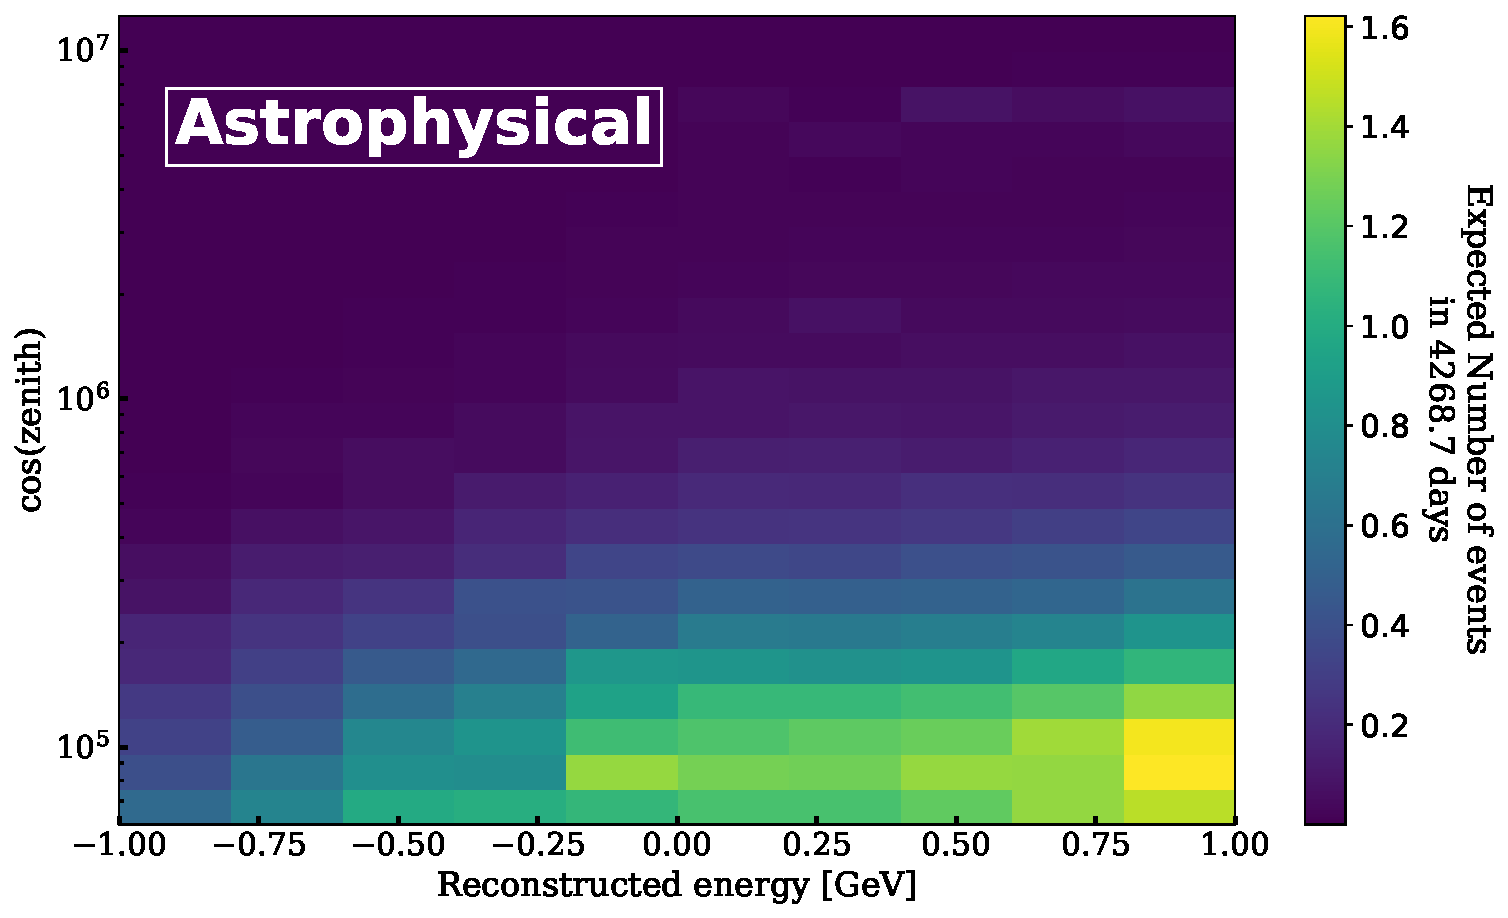
\includegraphics{./figures/Analysis/Cascades_Astrophysical.pdf}
    \end{subfigure}
    \hfill
    \begin{subfigure}[h]{0.72\textwidth}
        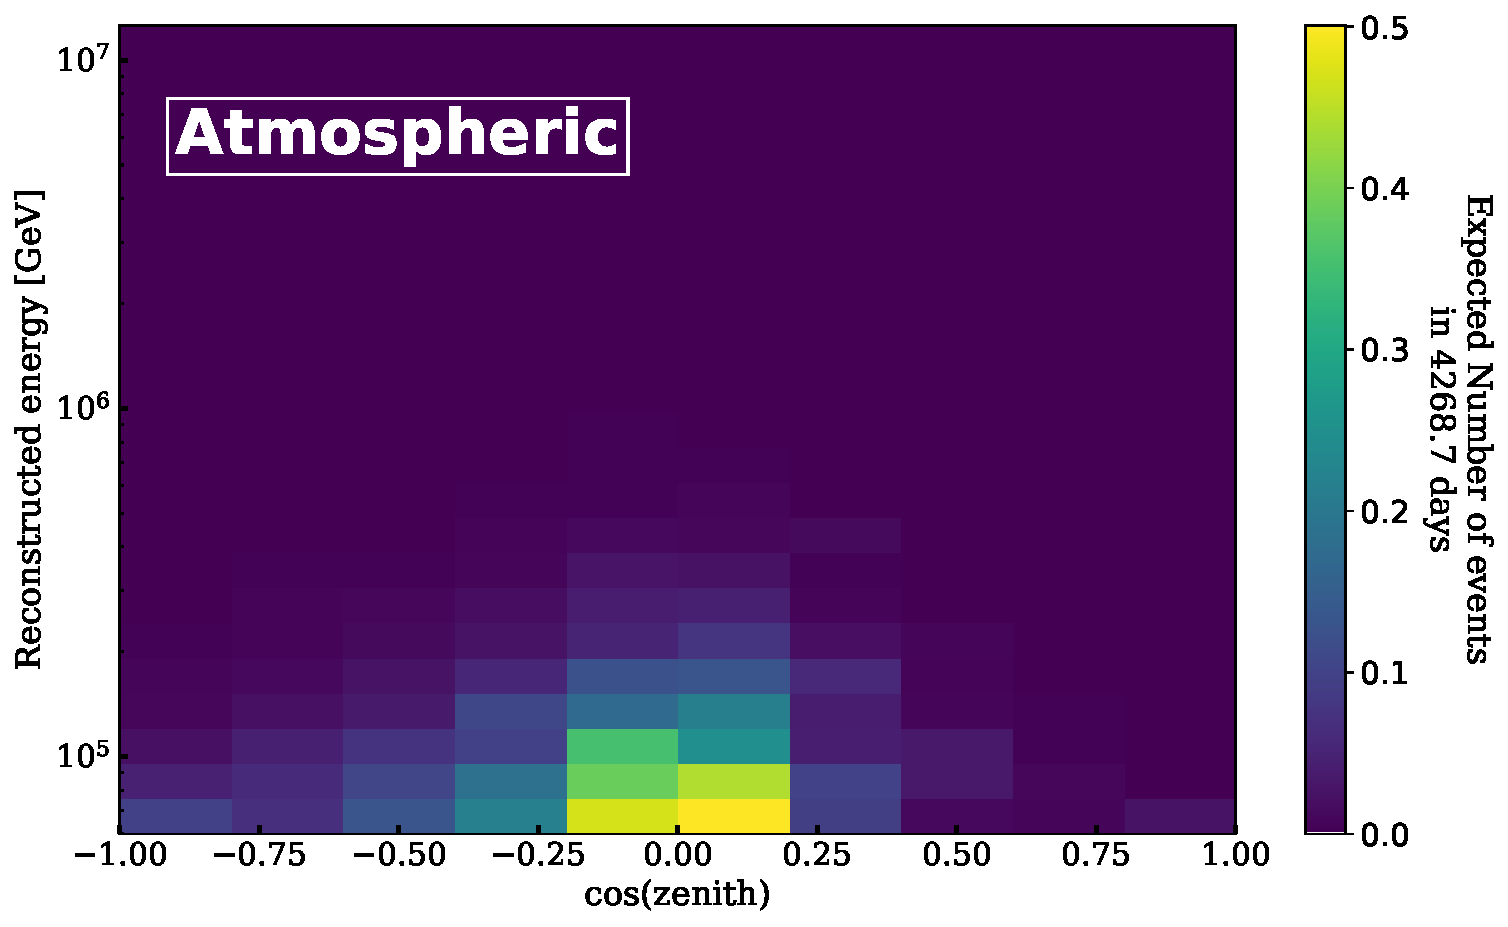
\includegraphics{./figures/Analysis/Cascades_Atmospheric.pdf}
       
    \end{subfigure}%
    \caption{2D Monte Carlo templates, constructed using reconstructed total energy ($E_{\text{Tot}}$) and reconstructed zenith ($\cos(\theta_z)$) for events classified as \textbf{single cascades}. The signal (left), representing \emph{Astrophysical neutrinos} of the sample and the background (right), representing \emph{Atmospheric neutrinos}, including conventional, prompt and single muon fluxes.}
    \labfig{cascades_2d}
\end{figure*}

\begin{figure*}[h!]
    \begin{subfigure}[h]{0.72\textwidth}
        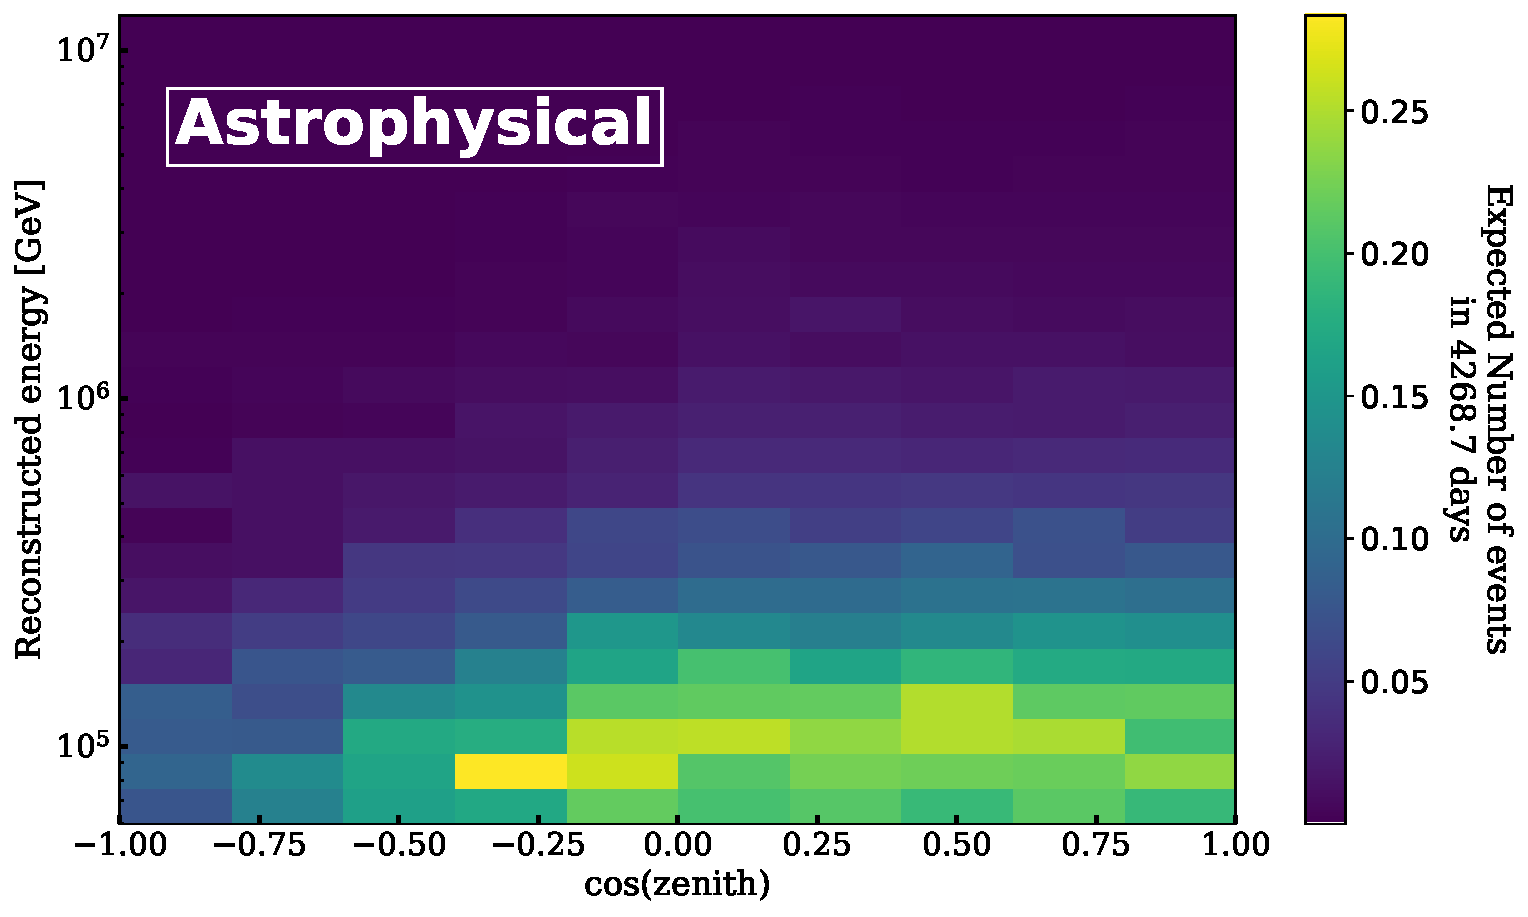
\includegraphics{./figures/Analysis/Tracks_Astrophysical.pdf}
    \end{subfigure}
    \hfill
    \begin{subfigure}[h]{0.72\textwidth}
        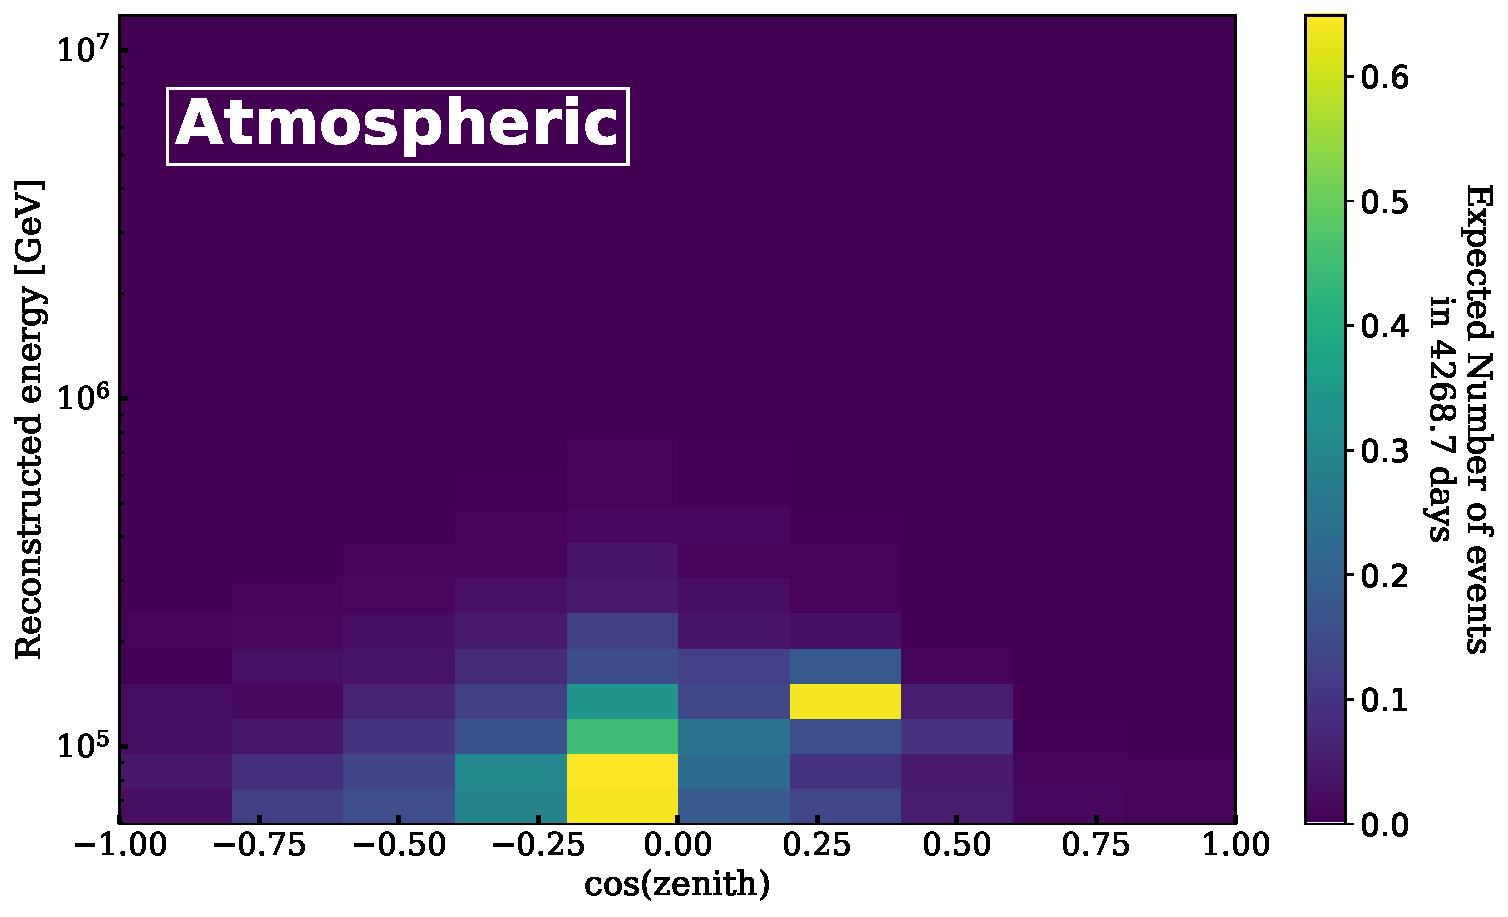
\includegraphics{./figures/Analysis/Tracks_Atmospheric.pdf}
       
    \end{subfigure}%
    \caption{2D Monte Carlo templates, constructed using reconstructed total energy ($E_{\text{Tot}}$) and reconstructed zenith ($\cos(\theta_z)$) for events classified as \textbf{tracks}. The signal (left), representing \emph{Astrophysical neutrinos} of the sample and the background (right), representing \emph{Atmospheric neutrinos}, including conventional, prompt and single muon fluxes.}
    \labfig{tracks_2d}
\end{figure*}

This becomes more evident in one dimensional distribution for both of these subsamples (\reffig{cascade_mc} for cascades and \reffig{tracks_mc} for tracks), where total expectation is broken down in individual flux contributions (as desribed in \ref{sec:params}). In case of Energy distribution of single cascades (right panel of \reffig{cascade_mc}), except for lower energy bins (up to $\sim110$ TeV), astrophysical single cascade events dominates. Glashow peak due to $\bar{\nu}_e$ is clearly visible too. Note the missong muon component, due to lack of enough \texttt{MUONGUN} simulation, as described in \ref{sec:params}. For Tracks (\reffig{tracks_mc}), although there is a similar supression due to self veto effects, but the constribution of single muons, simulated using \texttt{MUONGUN} events, is clearly visible, dominating in the same down-going region. As described before, the template is noisey due to large monte carlo uncertainties. In general, tracks sample shows larger contribution due to atmospheric fluxes compared to single cascades\sidenote{recall that single cascades also show contributions from all flavour Neutral Current (NC) interactions}. Similar 1 dimensional distributions of $\mathrm{L}_{\mathrm{dc}}$ and $\mathrm{E}_{\mathrm{Tot}}$ are shown for completeness, but as described before, double cascades do not show any striking differences going from astrophysical to atmopsheric fluxes as background is due to $\nu_{e}$ and $\nu_{\mu}$ events.


\begin{figure*}[h!]
    \caption{One dimensional observable distribution, for HESE Single Cascades showing expected number of events as a function of reconstructed energy (right) and reconstructed zenith (left), broken down into different flux components. Only statistical errors are shown.}
    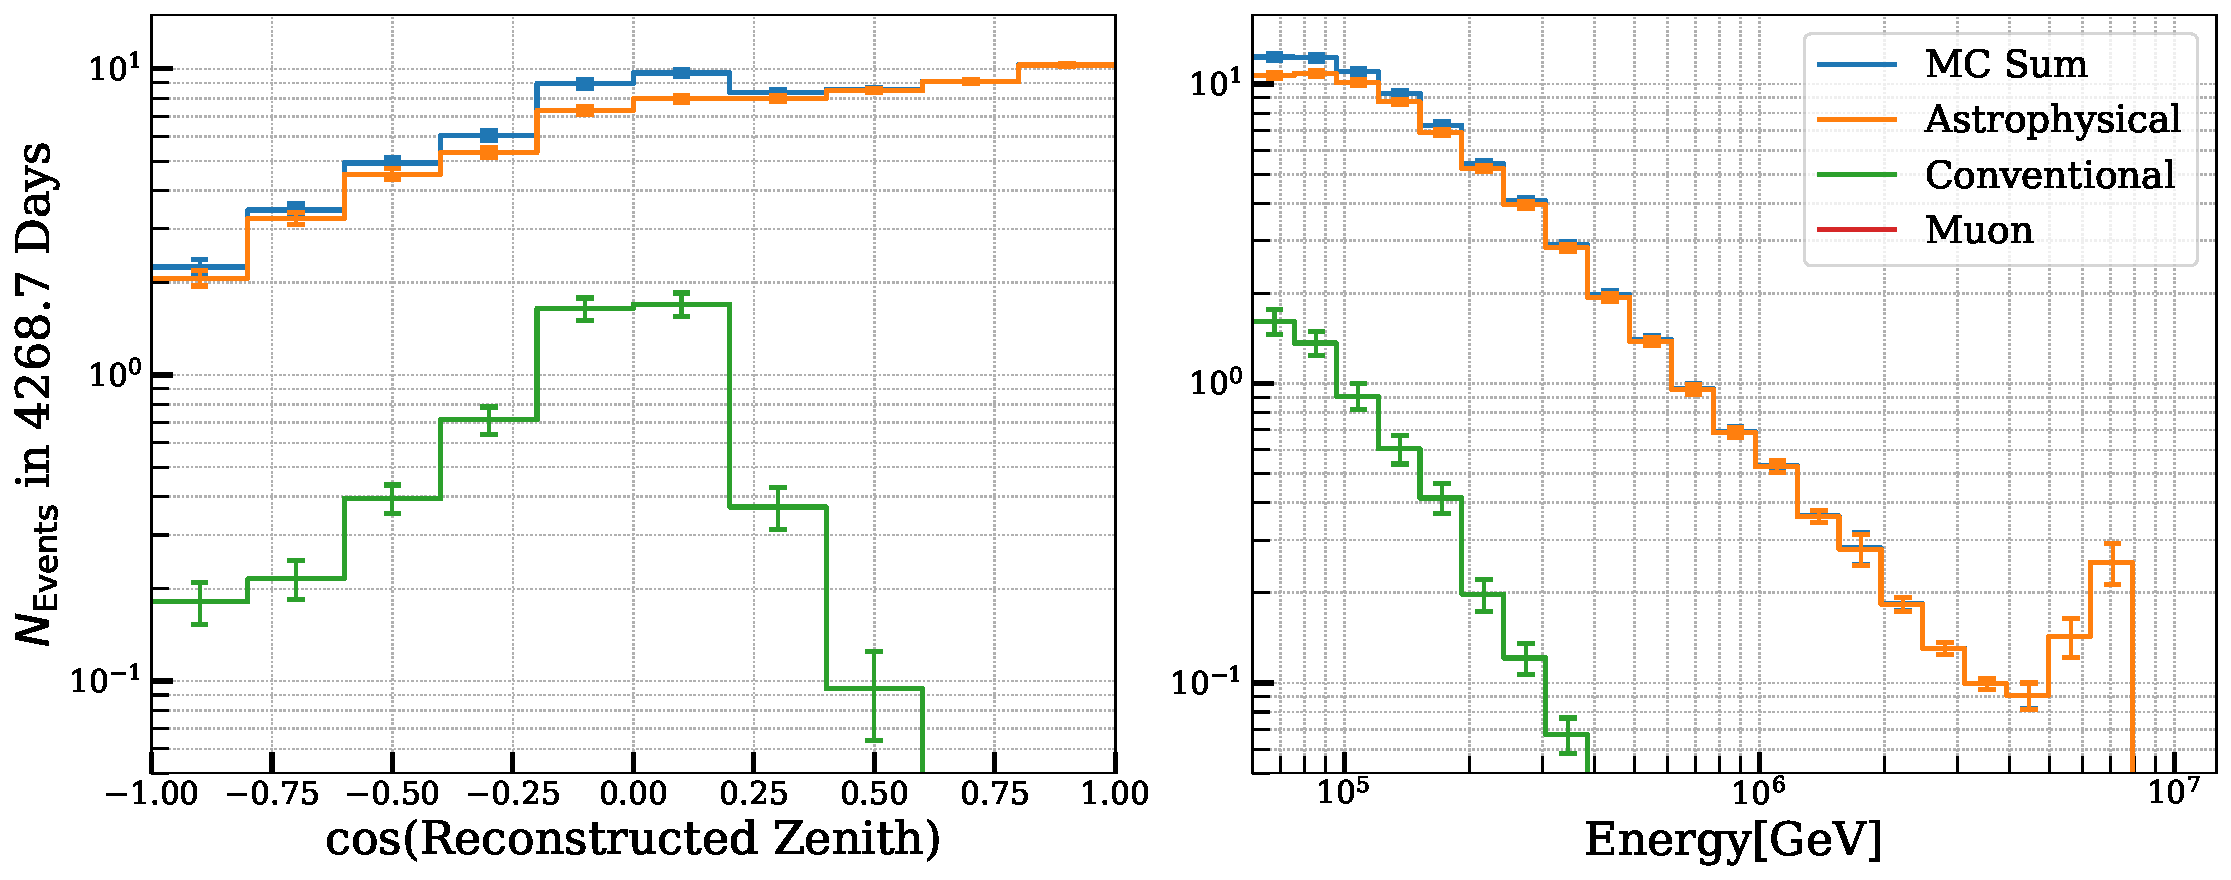
\includegraphics{./figures/Analysis/Cascades.pdf}
    \labfig{cascade_mc}
\end{figure*}

\begin{figure*}[h!]
    \caption{One dimensional observable distribution, for HESE Tracks showing expected number of events as a function of reconstructed energy (right) and reconstructed zenith (left), broken down into different flux components. Only statistical errors are shown.}
    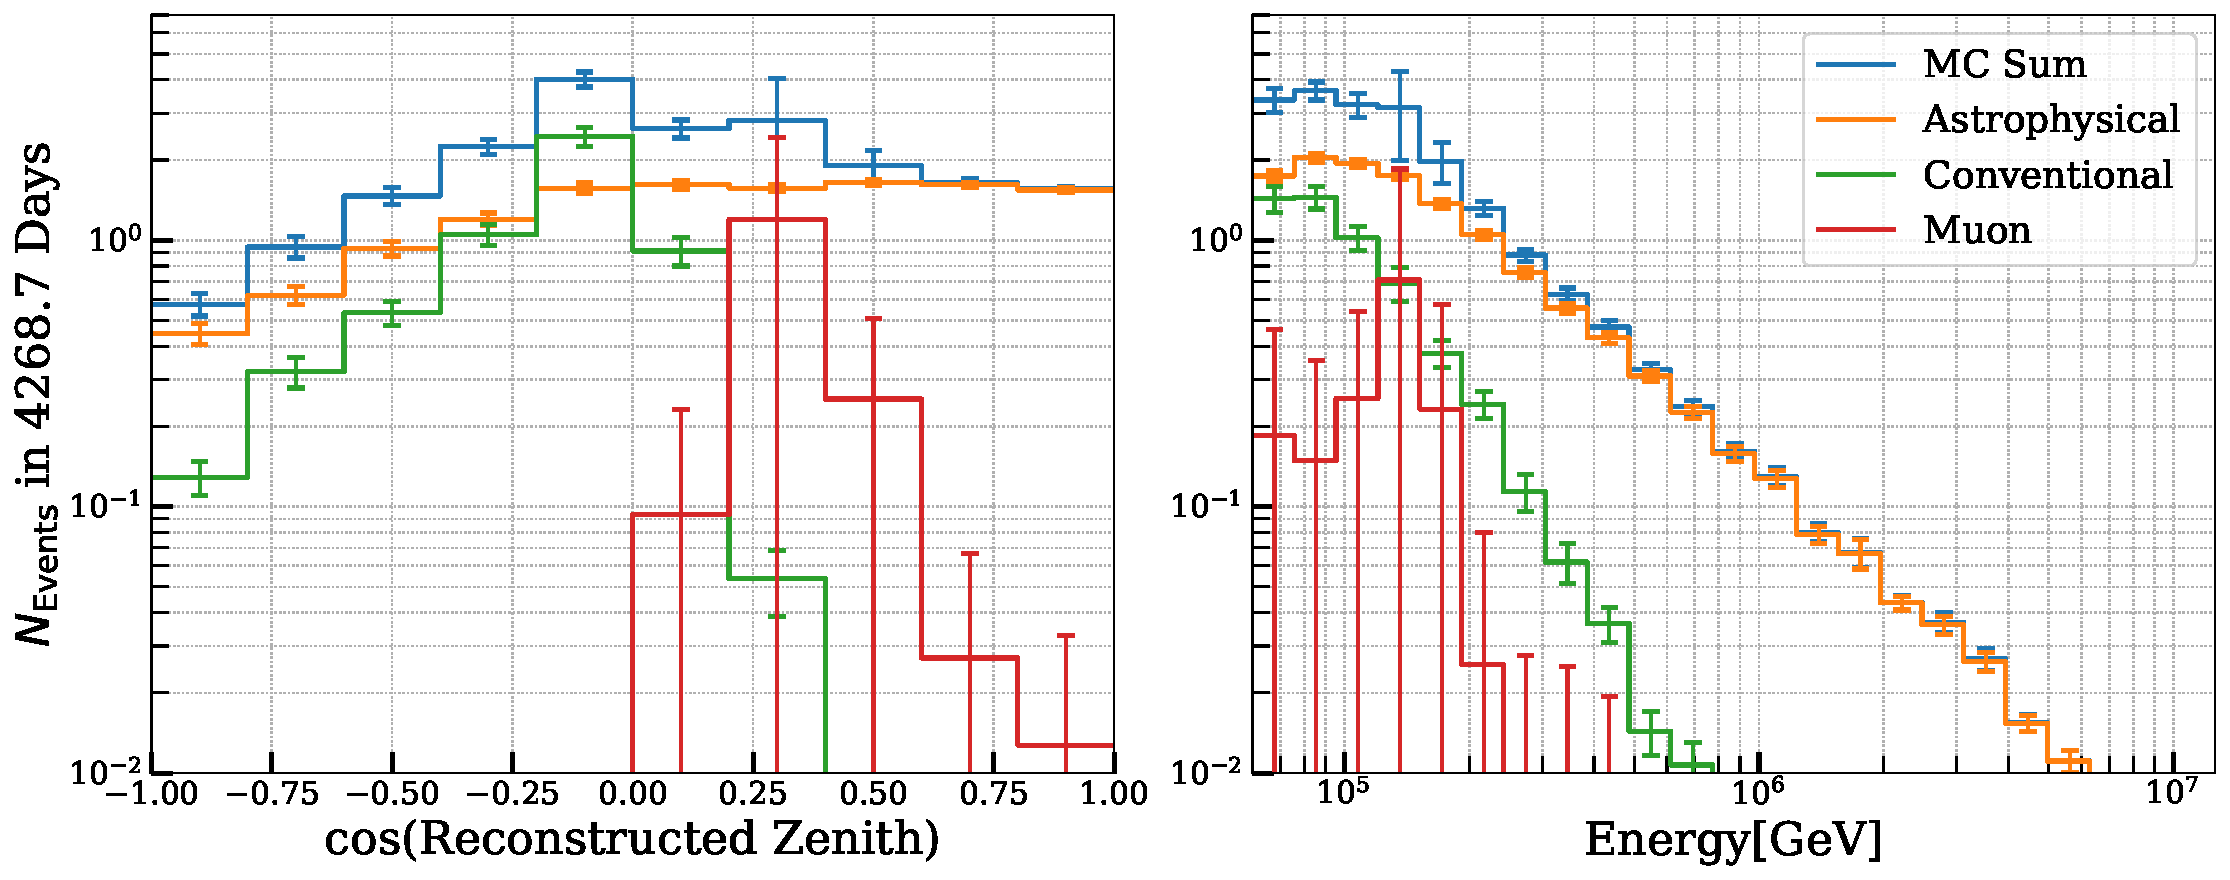
\includegraphics{./figures/Analysis/Tracks.pdf}
    \labfig{tracks_mc}
\end{figure*}

\begin{figure*}[h!]
    \caption{One dimensional observable distribution, for HESE DOuble Cascades showing expected number of events as a function of reconstructed energy (right) and reconstructed tau decay length (left), broken down into different flux components. Only statistical errors are shown.}
    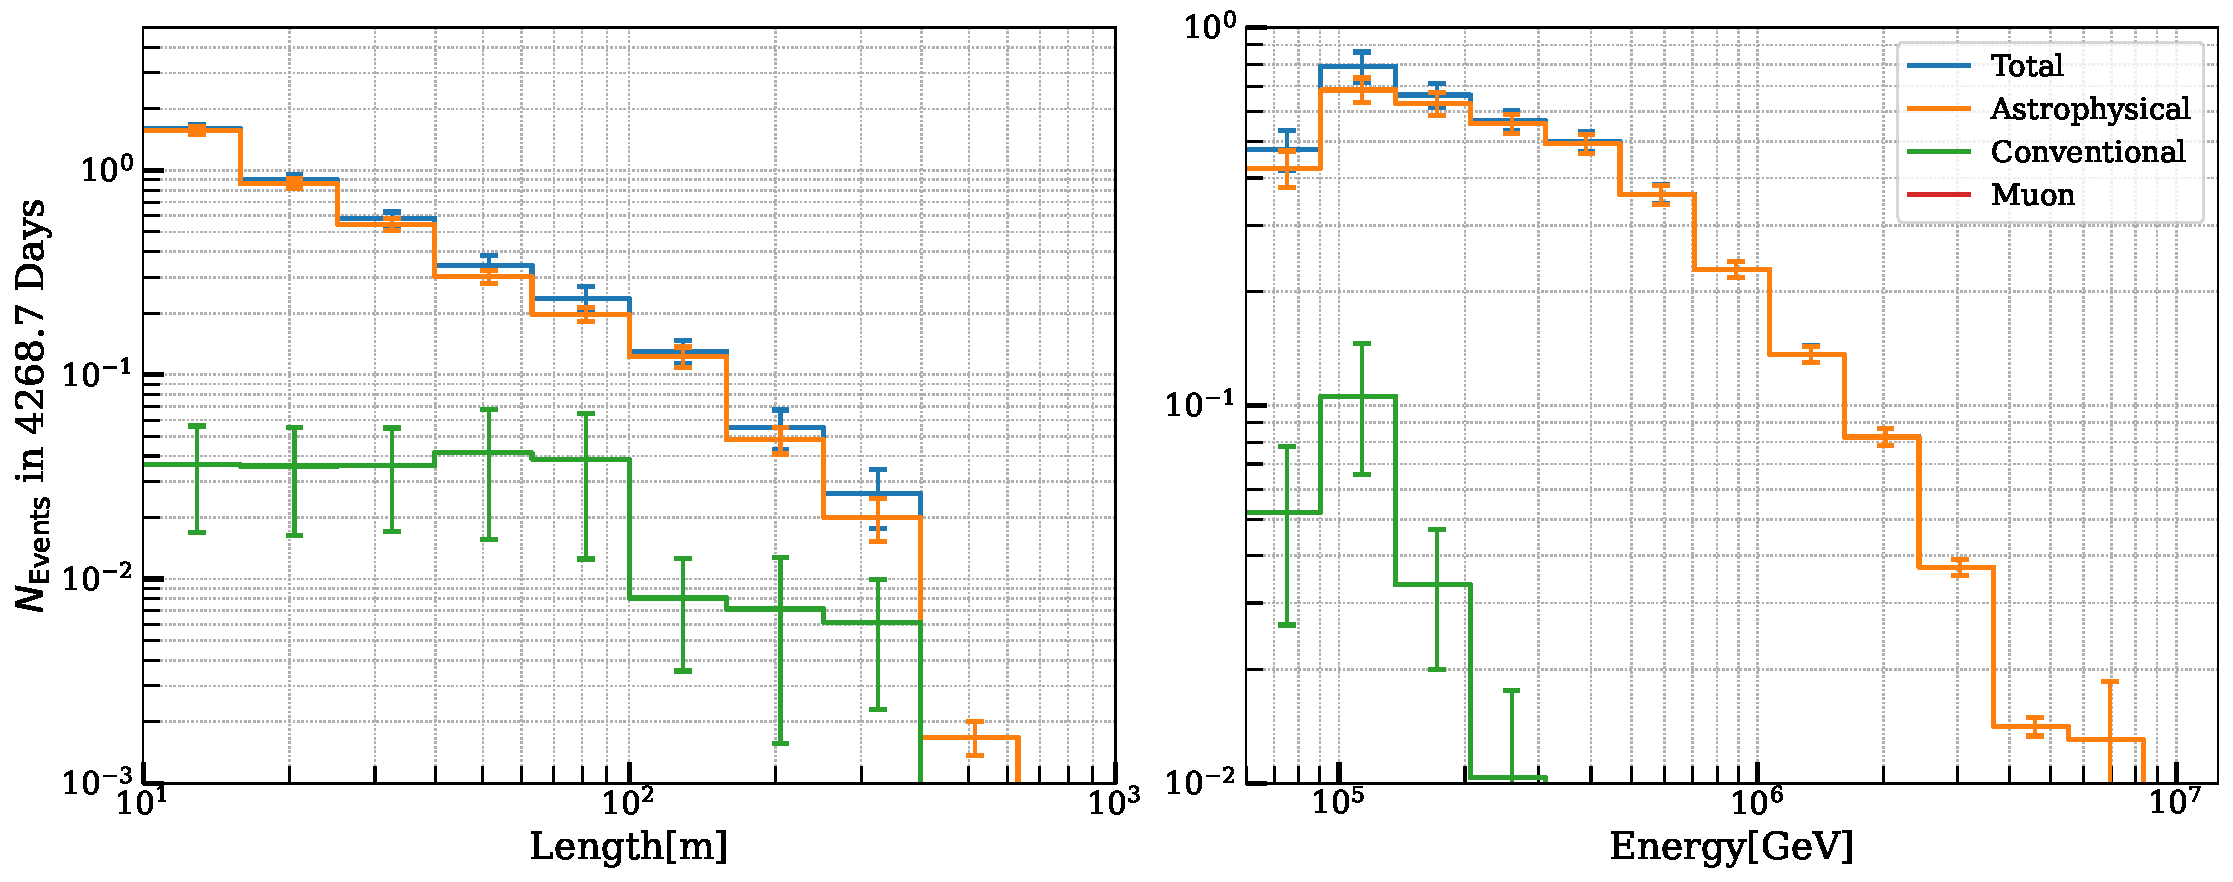
\includegraphics{./figures/Analysis/Double.pdf}
    \labfig{double_mc}
\end{figure*}

\section{Analysis Sensitivity}
\label{sec:sensitivty}
All fits and related calculations are carried out using a software toolkit called \textbf{\texttt{NNMFit}}. Developed within the IceCube collaboration, \texttt{NNMFit} has been applied in many other IceCube analyses. Essentially, the toolkit handles the statistical modeling required for forward-folding fits using high-energy neutrino data with binned likelihoods. It supports Monte Carlo event weighting, testing various flux models using signal and nuisance parameters, applying systematic detector uncertainties, and performing fits to data. The toolkit also enables joint fitting across different event selections. The \texttt{aesara} backend allows fast and efficient forward folding of Monte Carlo samples, even for large datasets, and offers automated differentiation that greatly assists in optimizing likelihood functions. More details on this toolkit are found in \sidecite{richard_thesis}.\todo{any other thesis/paper/links required??}

Using all the ingredients in the form of fluxes constructed from signal and nuisance parameters, and following the described method, the flavor composition parameter space is scanned to obtain a two-dimensional confidence region for the flavor composition, as shown in \reffig{sensitivity}. To derive these limits, an Asimov dataset is constructed (see Section~\ref{sec:analysis}), assuming the benchmark astrophysical neutrino spectrum given in \ref{eq:SPL}. All other nuisance parameters are fixed at their baseline values listed in \reftab{fit_params}. The astrophysical neutrino flavor composition is constrained by evaluating the likelihood ratio in a profile likelihood scan, with confidence regions estimated using Wilks’s theorem. The expected number of events over 12 years of HESE data, assuming the spectrum in \ref{eq:SPL}, is broken down by flux components and shown in Monte Carlo templates in \reftab{expected_events}. The fitting procedure bins all HESE events above 60 TeV in reconstructed energy and further categorizes them into three subsamples based on morphology: single cascades, tracks, and double cascades. Each sample is fit using 2D Monte Carlo templates, with the appropriate analysis variables shown in \reffig{cascades_2d}, \reffig{tracks_2d}, and \reffig{LvsE_signalbkg}.

\begin{table}[h]
    \caption{The expected number of events from different flux components for the $\sim12$ years of HESE sample,  broken down for each individual fluxes, for single cascades, double cascades, and tracks categories. Only Monte Carlo uncertainties are included. The astrophysical spectrum assumed follows Equation~\ref{eq
    }}
    \labtab{fit_params}
    
    \begin{tabular}{ c |c|c|c}
        
        \hline
        &Single Cascades &Double Cascades&Tracks\\
        \hline
        \hline
        Astrophysical&$67\pm1$& $4\pm0.2$ & $13\pm0.5$\\
        Conventional & $5\pm0.7$& $0.2\pm0.1$ &$5\pm0.6$\\
        Atm. Muons & - & - & $2\pm3$\\
        \hline
        MC Sum & $72\pm2$ & $4\pm0.3$ & $20\pm3$\\
        \hline
    \end{tabular}
\end{table}

\begin{figure}[h!]
    \caption{Sensitivity of the analysis presented in this thesis to measure the the flavor composition using $\sim12$ years of IceCube HESE data assuming single power law given in Equation~\ref{eq:SPL}, with flavour composition of $\nu_e:\nu_{\mu}:\nu_{\tau}=1:1:1$. Contours show the $1\sigma$ (solid) and $2\sigma$ (dashed) confidence intervals assuming Wilks' theorem.}
    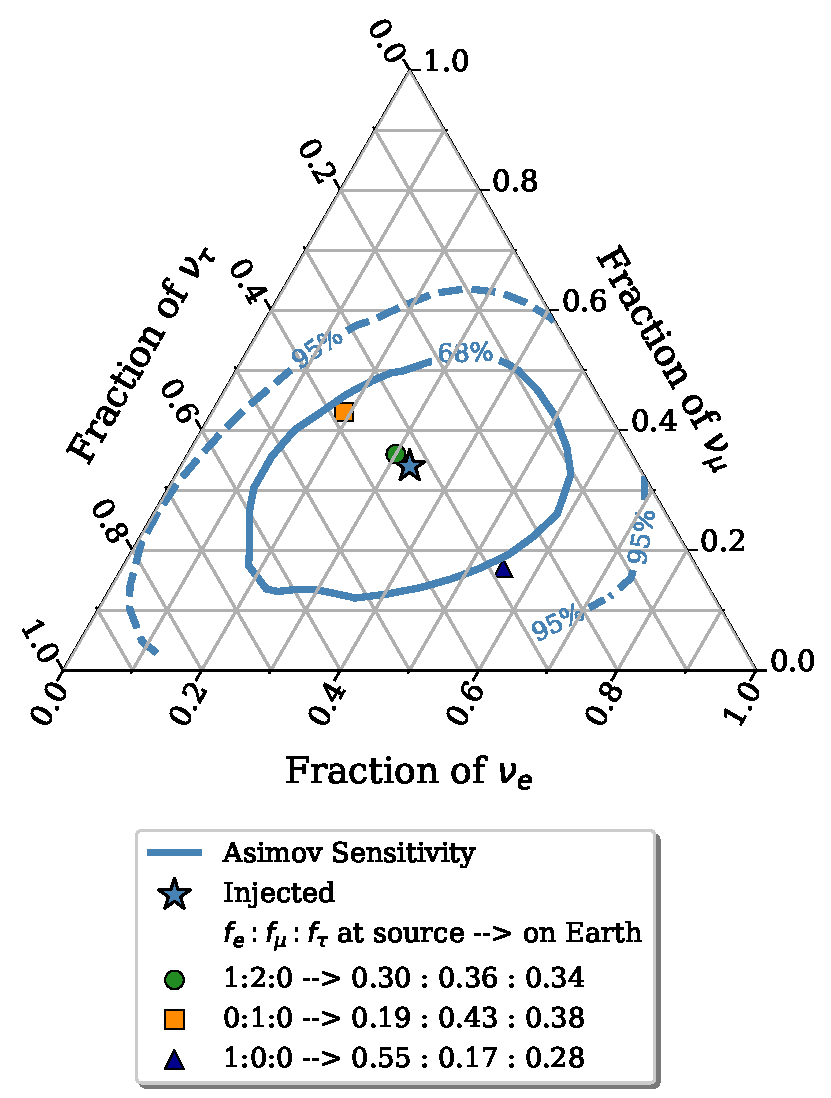
\includegraphics{./figures/Analysis/Asimov_Sensitivity.pdf}
    \labfig{sensitivity}
\end{figure}

The sensitivity results in \reffig{sensitivity} reveal that none of the standard source scenarios discussed in \ref{sec:flavor_theory} can be rejected with high significance. For instance, the neutron beam scenario (represented by the dark blue triangle) is barely excluded at the $\sim1\sigma$ level. It is important to recall that the sensitivity of this analysis to the astrophysical tau-neutrino flux depends strongly on the assumed spectral shape of the neutrino flux. This sensitivity arises from the energy-dependent identification efficiency of tau-neutrino interactions. At higher energies, more energy is transferred to the secondary tau, increasing its decay length and enhancing identification efficiency. A softer spectrum, however, leads to more tau-neutrino interactions at lower energies, where they are harder to identify. Additionally, the sudden disappearance of line segments in the 95\% confidence contours, particularly in regions where the $\nu_\mu$ fraction approaches zero, is a result of the flavor fit parameterization (see Equation \ref{eq:flav_frac}). By construction, this fraction cannot be zero, meaning that this phase space is inaccessible to the fit.

While earlier versions of this analysis explored alternative flux models (or example, a broken power law introduces a break in the conventional single power law, resulting in different spectral indices on either side of the break energy), this was not done here. The decision was based from recent findings from another IceCube analysis that combined two other event samples (Tracks and Cascades), revealing features in the extragalactic astrophysical neutrino spectrum targetting much larger range of Neutrino energies ($\sim10$ TeV to $\sim10$ PeV) \sidecite{globalfit_icrc}. That study provided evidence of a spectral break at around 24 TeV with more than $4\sigma$ significance. The spectrum showed hardness below this break, followed by softening at higher energies, consistent with the softer spectral measurement from HESE-7.5, which targets the higher-energy range. Importantly, this high-statistics analysis, which extends well beyond the energy range of the current analysis, found no significant structures at HESE energies. Furthermore, an independent study using a different event sample \sidecite{MESE_ICRC} reported similar spectral features and closely aligned best-fit values, solidifying the argument even more. 

